\documentclass[../../main.tex]{subfiles}

\graphicspath{{../../fig/}}
\setcounter{section}{0}

\begin{document}
\chapter{スパースワイヤーグリッドのたわみ量の評価}
\label{chap:wiresag_swg}
\ref{chap:wiresag}章にて、ワイヤーのたわみ量を自動で評価する装置を開発した。
本章では、開発した装置を用いて実際に偏光角較正に使用されるスパースワイヤーグリッドのたわみ量を評価する。
はじめに、評価するスパースワイヤーグリッドの作成方法について述べ、次いで評価結果とその考察を行う。
その後、評価されたたわみ量が大きかったものについて修繕を加え、再度評価を行った結果について述べる。
最後に、今回のたわみ量の評価を通じて得られた、スパースワイヤーグリッドの作成方法に関する今後の展望について述べる。

\section{評価されたスパースワイヤーグリッドの詳細}
今回評価したスパースワイヤーグリッドは、\ref{subsec:wg_design}項で述べたように$\SI{230}{g}$の重りを使用し、
ワイヤー番号が奇数番目のものと偶数番目のものに分け、二回に分けてワイヤーを張ることで作成された。
このとき、はじめにワイヤー番号が奇数番目のものを張り、次にワイヤー番号が偶数番目のものを張った。
作成されたスパースワイヤーグリッドを装置に取り付けた様子を図\ref{fig:wiresag_swg_sparse_wiregrid}に示す。
なお、\ref{chap:wiresag}章にて述べたように一度に測定できるのはスパースワイヤーグリッドの半面のみであるので、
ワイヤー番号が$0\sim19$番のワイヤーと$20\sim38$番のワイヤーに分けて測定を行った。
\begin{figure}[H]
    \centering
    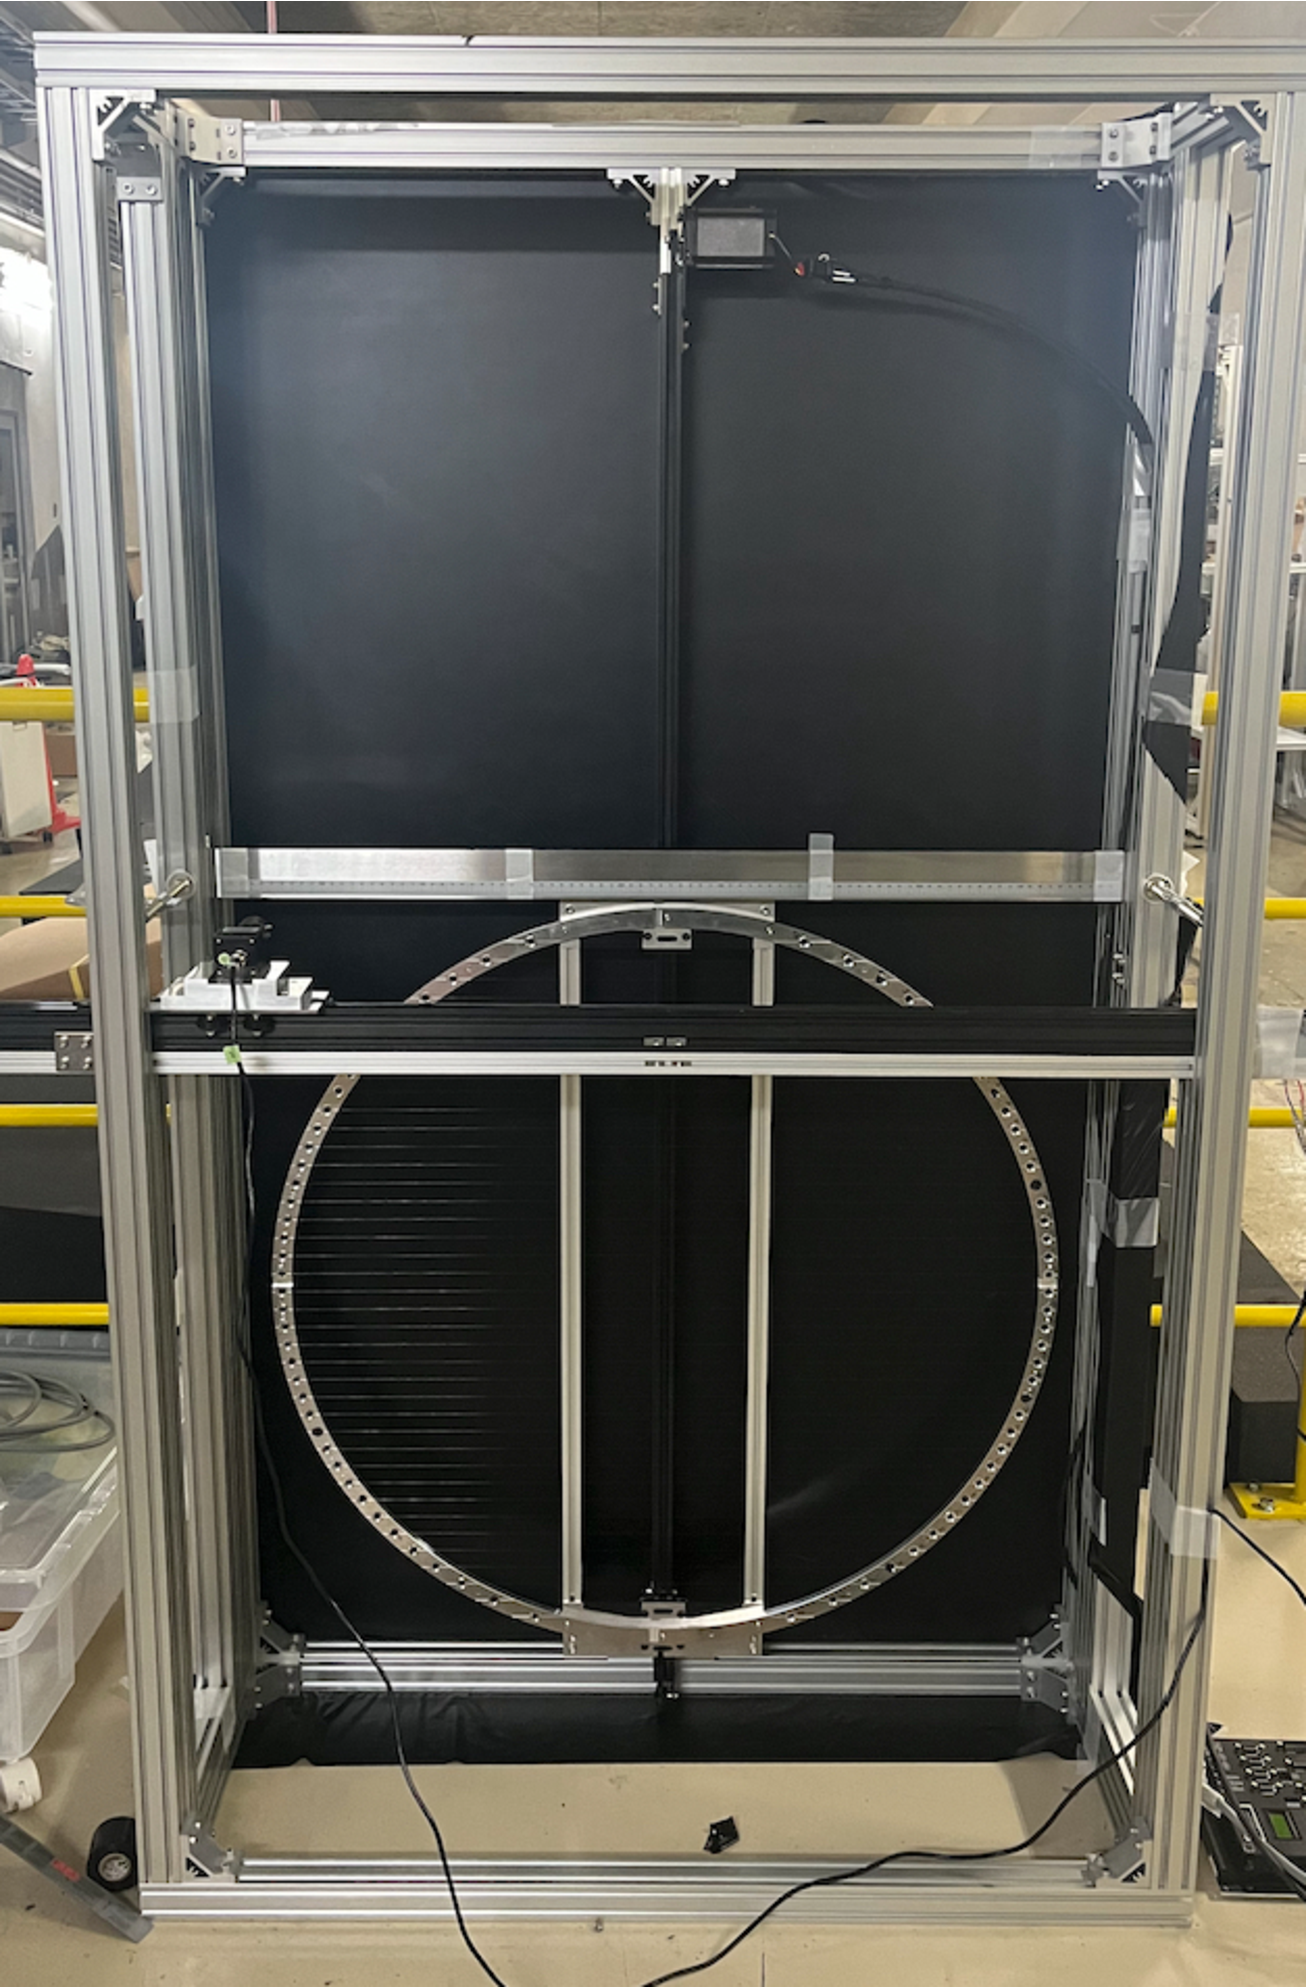
\includegraphics[width=0.4\textwidth]{wiresag_swg/wiresag_sparse_wiregrid.pdf}
    \caption{スパースワイヤーグリッドのたわみ量の評価の様子}
    \label{fig:wiresag_swg_sparse_wiregrid}
\end{figure}
\section{評価結果とその考察}
図\ref{fig:wiresag_swg_result}(\subref{fig:wiresag_swg_sag_result})にスパースワイヤーグリッドのたわみ量の評価結果を示す。
横軸はワイヤー番号、縦軸はワイヤーのたわみ量を示している。
fitting errorを統計的な誤差として、前章にて得られた$\SI{50}{\mu m}$を系統的な誤差として、それらの2乗和をたわみ量の誤差として示した。
図中には測定されたたわみ量に加え、理論値として$\SI{230}{g}$の重りによって生まれるたわみ量を、
たわみ角が$0.3\tcdegree,\,0.5\tcdegree$になるたわみ量を示している。
図\ref{fig:wiresag_swg_result}(\subref{fig:wiresag_swg_sag_angle_result})に
評価されたたわみ量をたわみ角に変換した結果を示す。
横軸はワイヤー番号、縦軸はワイヤーのたわみ角を示している。
図中には測定されたたわみ角に加え、たわみ角が$0.03\tcdegree,\,0.05\tcdegree$の線を示している。
測定されたたわみ角の平均は$0.025\tcdegree$であり、たわみ角の誤差の平均は$0.011\tcdegree$であった。
したがって、ワイヤーのたわみ角が与える望遠鏡の偏光角較正への影響は、$0.036\tcdegree$であり、$<0.04\tcdegree$である。 
これは先行研究が与えた$<0.05\tcdegree$よりも小さい値である。

得られたたわみ量は先行研究よりも小さい値であったが、明らかにたわみ量が大きいワイヤーが存在しており、
さらにワイヤー番号が奇数か偶数かによってたわみ量の値が異なっている。
図\ref{fig:wiresag_swg_even_odd}にワイヤー番号の偶奇によるたわみ量の違いを示す。
偶数番目のワイヤーのたわみ量を青点で示し、奇数番目のワイヤーのたわみ量を橙点で示している。
この図より、奇数番目のワイヤーのたわみ量が大きいことがわかる。
今回評価したスパースワイヤーグリッドは奇数番目のワイヤーから張り始めたことから、このたわみ量の違いは、
\begin{enumerate}
    \item 単に奇数番目のワイヤーを張るときにうまく張れなかった
    \item 後に張ったワイヤーにより、先に張ったワイヤーがたわんでしまった
\end{enumerate}
の2つの原因が考えられる。
そこで奇数番目のワイヤーのみを張り直し、修繕することによりたわみ量がどう変化するかを調べる。
\begin{figure}[H]
    \begin{minipage}[b]{0.5\hsize}
        \centering
        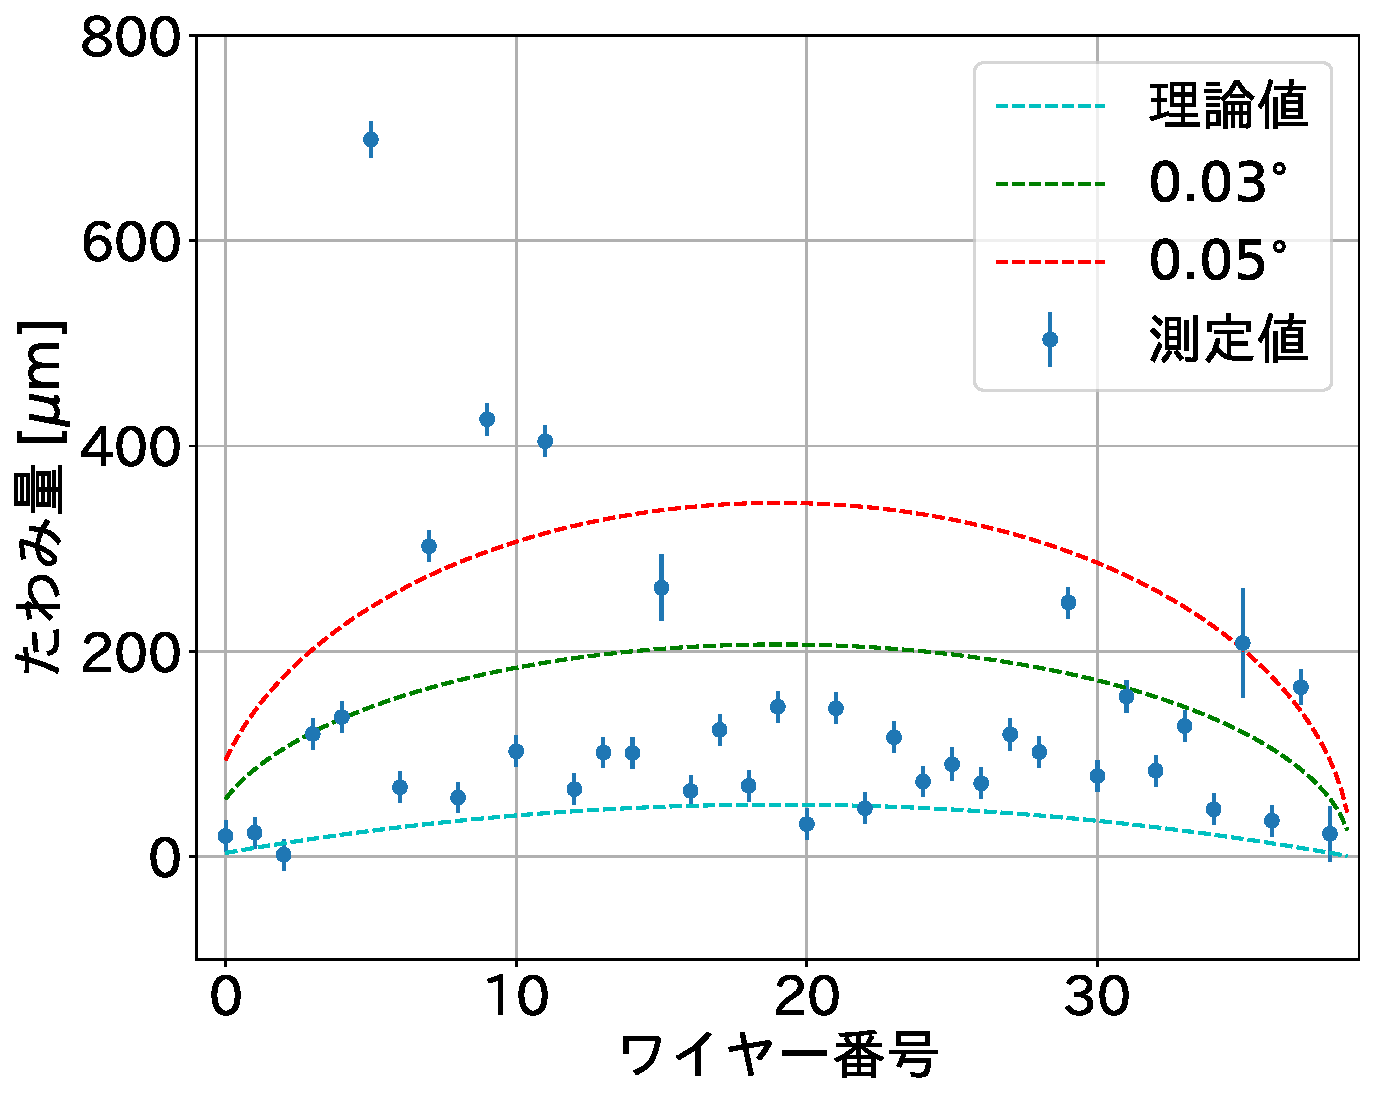
\includegraphics[width=1.0\textwidth]{wiresag_swg/swg_sag_before.pdf}
        \subcaption{}
        \label{fig:wiresag_swg_sag_result}
    \end{minipage}
    \begin{minipage}[b]{0.5\hsize}
        \centering
        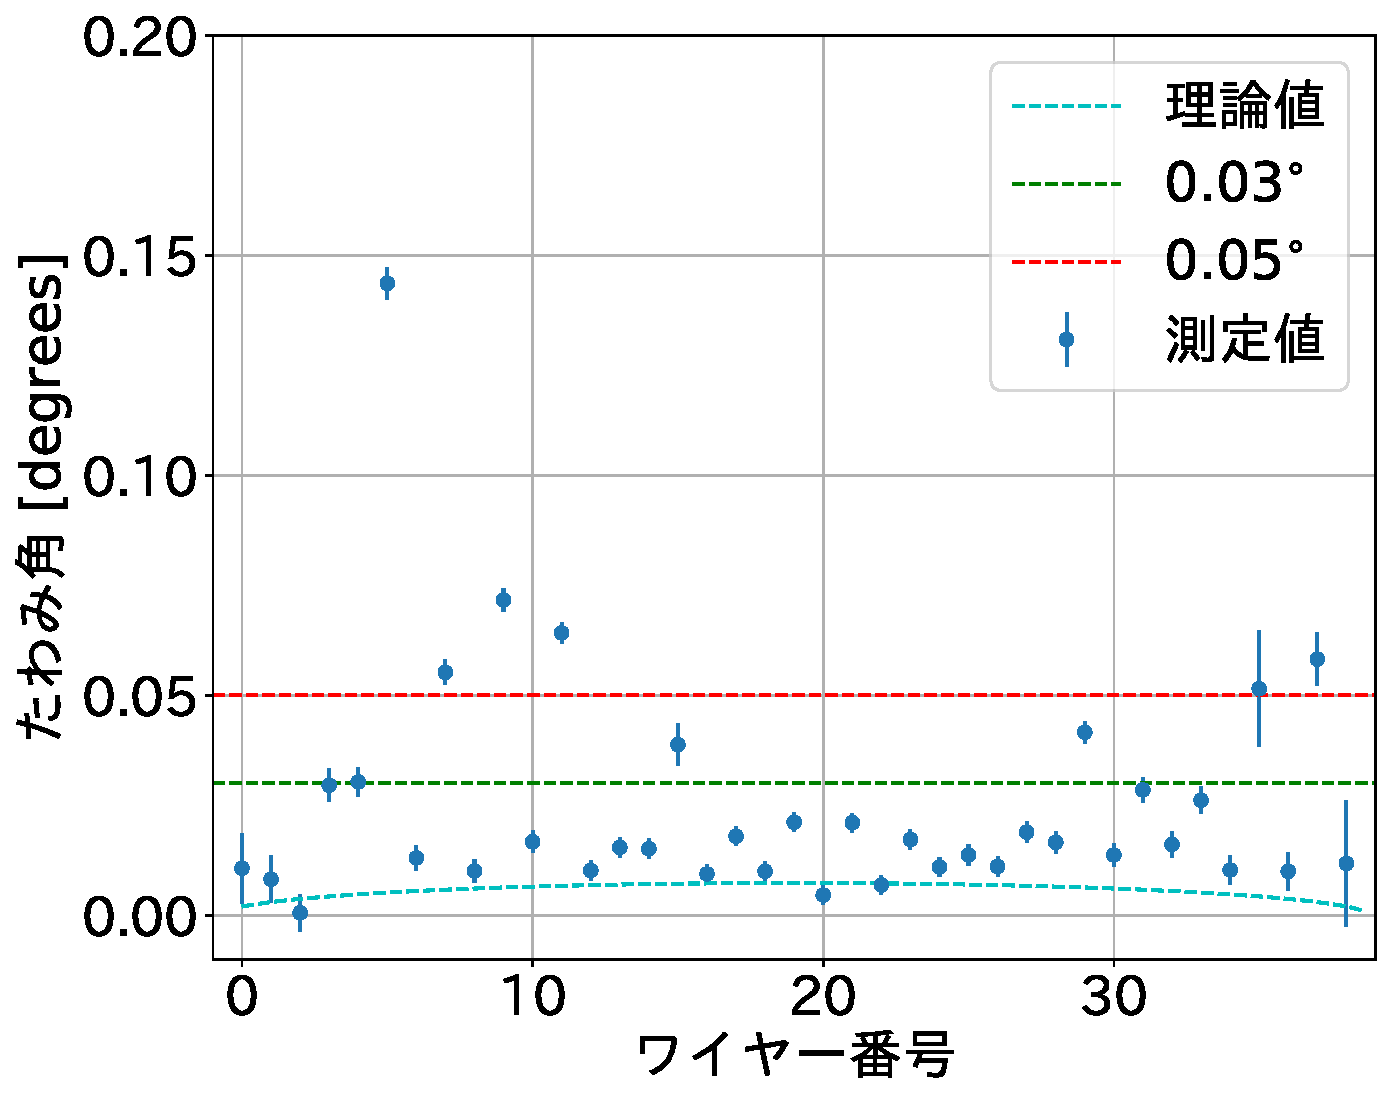
\includegraphics[width=1.0\textwidth]{wiresag_swg/swg_sag_angle_before.pdf}
        \subcaption{}
        \label{fig:wiresag_swg_sag_angle_result}
    \end{minipage}
    \caption{(\subref{fig:wiresag_swg_sag_result}) スパースワイヤーグリッドのたわみ量の評価結果\ 
             (\subref{fig:wiresag_swg_sag_angle_result}) スパースワイヤーグリッドのたわみ角の評価結果}
    \label{fig:wiresag_swg_result}
\end{figure}
\begin{figure}[H]
    \centering
    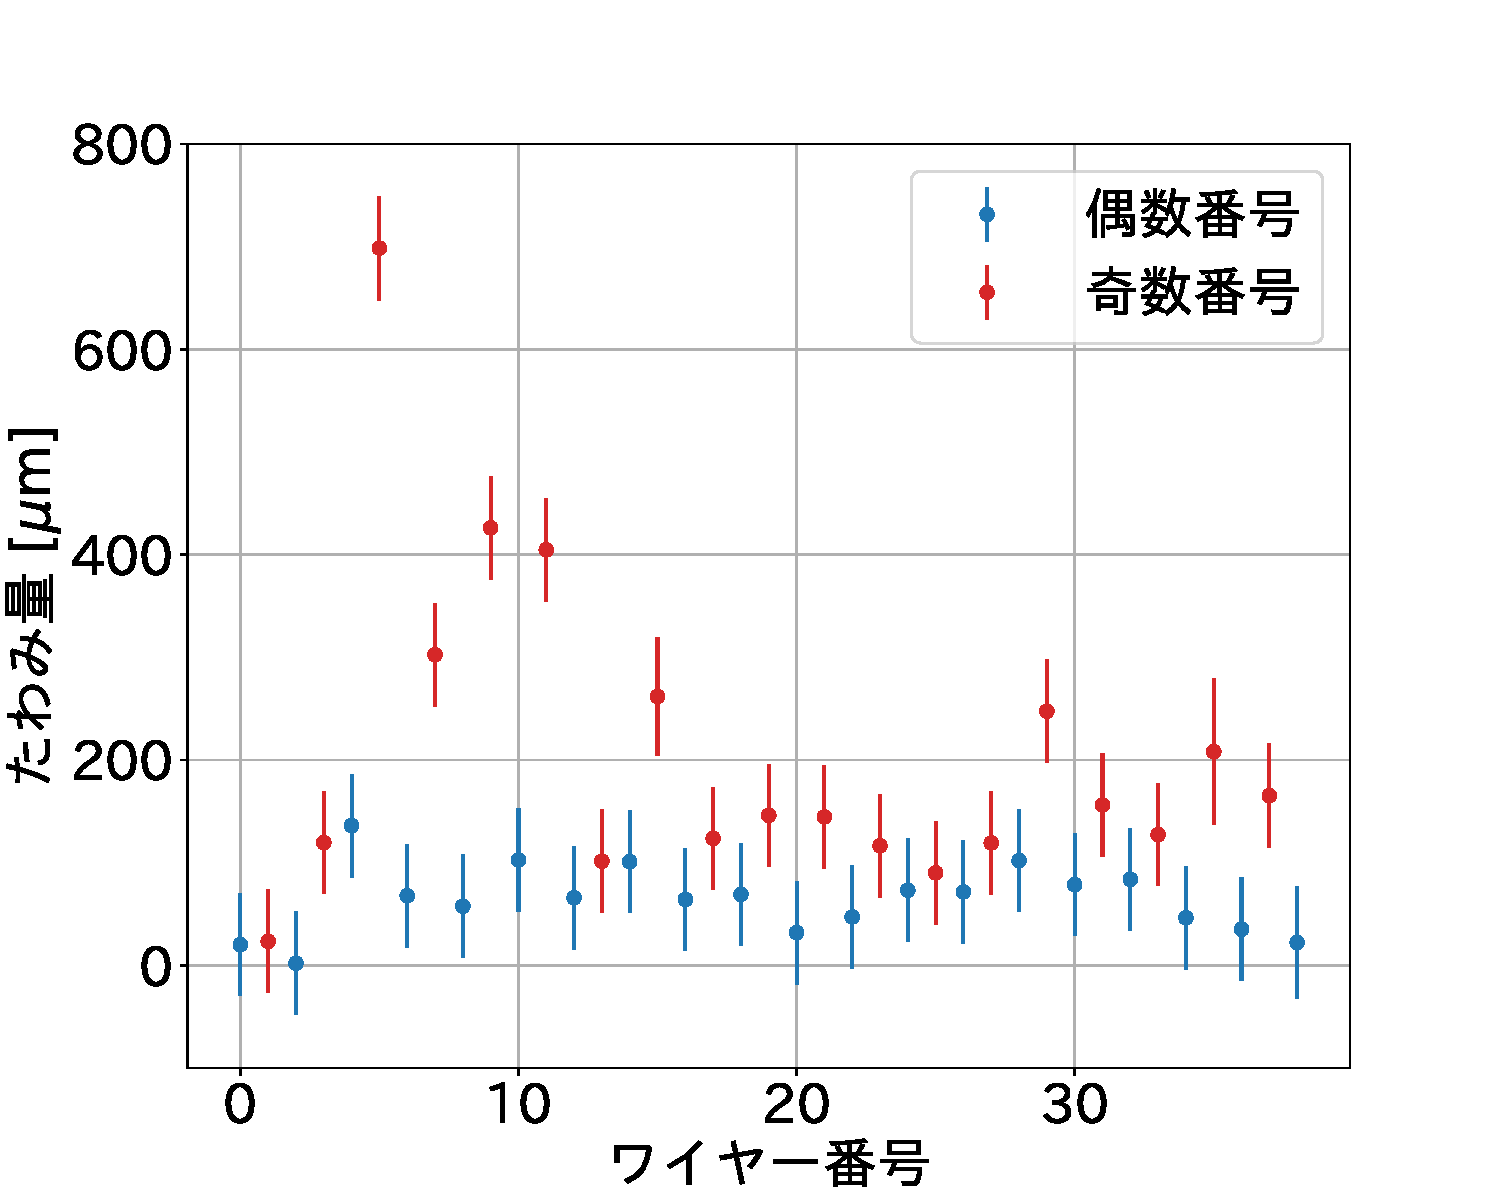
\includegraphics[width=0.8\textwidth]{wiresag_swg/swg_sag_before_even_odd.pdf}
    \caption{ワイヤー番号の偶奇によるたわみ量の違い}
    \label{fig:wiresag_swg_even_odd}    
\end{figure}

\section{修繕後のスパースワイヤーグリッドの評価}
修繕後のスパースワイヤーグリッドのたわみ量の評価結果を図\ref{fig:wiresag_swg_result_repair}(\subref{fig:wiresag_swg_sag_result_repair})に、
たわみ角の評価結果を図\ref{fig:wiresag_swg_result_repair}(\subref{fig:wiresag_swg_sag_angle_result_repair})に示す。
得られたたわみ角の平均は$0.02\tcdegree$であり、たわみ角の誤差の平均は$0.01\tcdegree$であった。
したがって、修繕後のワイヤーのたわみが与える望遠鏡の偏光角較正への影響は、$0.03\tcdegree$であり、修繕前の$0.036\tcdegree$よりも小さくなった。
この結果は、本装置を用いてワイヤーのたわみ量を評価することにより、品質の悪いワイヤーを張り直してたわみ量を改善可能であることを示している。

また、図\ref{fig:wiresag_swg_even_odd_repair}に修繕後のワイヤーについて、ワイヤー番号の偶奇によるたわみ量の違いを示す。
青点が偶数番目のワイヤーのたわみ量を示し、橙点が奇数番目のワイヤーのたわみ量を示している。
修繕後のワイヤーに関しては、奇数番目よりも偶数番目のワイヤーのたわみ量が大きくなっており、
修繕前の傾向と逆の傾向を示した。
図\ref{fig:wiresag_swg_even_odd_repair_comparison}(\subref{fig:wiresag_swg_sag_odd_comparison})に奇数番目のワイヤーのたわみ量を修繕前後で比較した結果を、
図\ref{fig:wiresag_swg_even_odd_repair_comparison}(\subref{fig:wiresag_swg_sag_even_comparison})に偶数番目のワイヤーのたわみ量を修繕前後で比較した結果を示す。
これらの図から、ワイヤーのたわみ量を修繕前後では奇数番目は修繕によりたわみ量が小さくなっているが、偶数番目は修繕後の方が大きくなっていることがわかる。
以上の結果から、スパースワイヤーグリッドのワイヤーは2回に分けて張ることにより、先に張られたワイヤーがたわんでしまう可能性があることがわかった。


\begin{figure}[H]
    \begin{minipage}[b]{0.5\hsize}
        \centering
        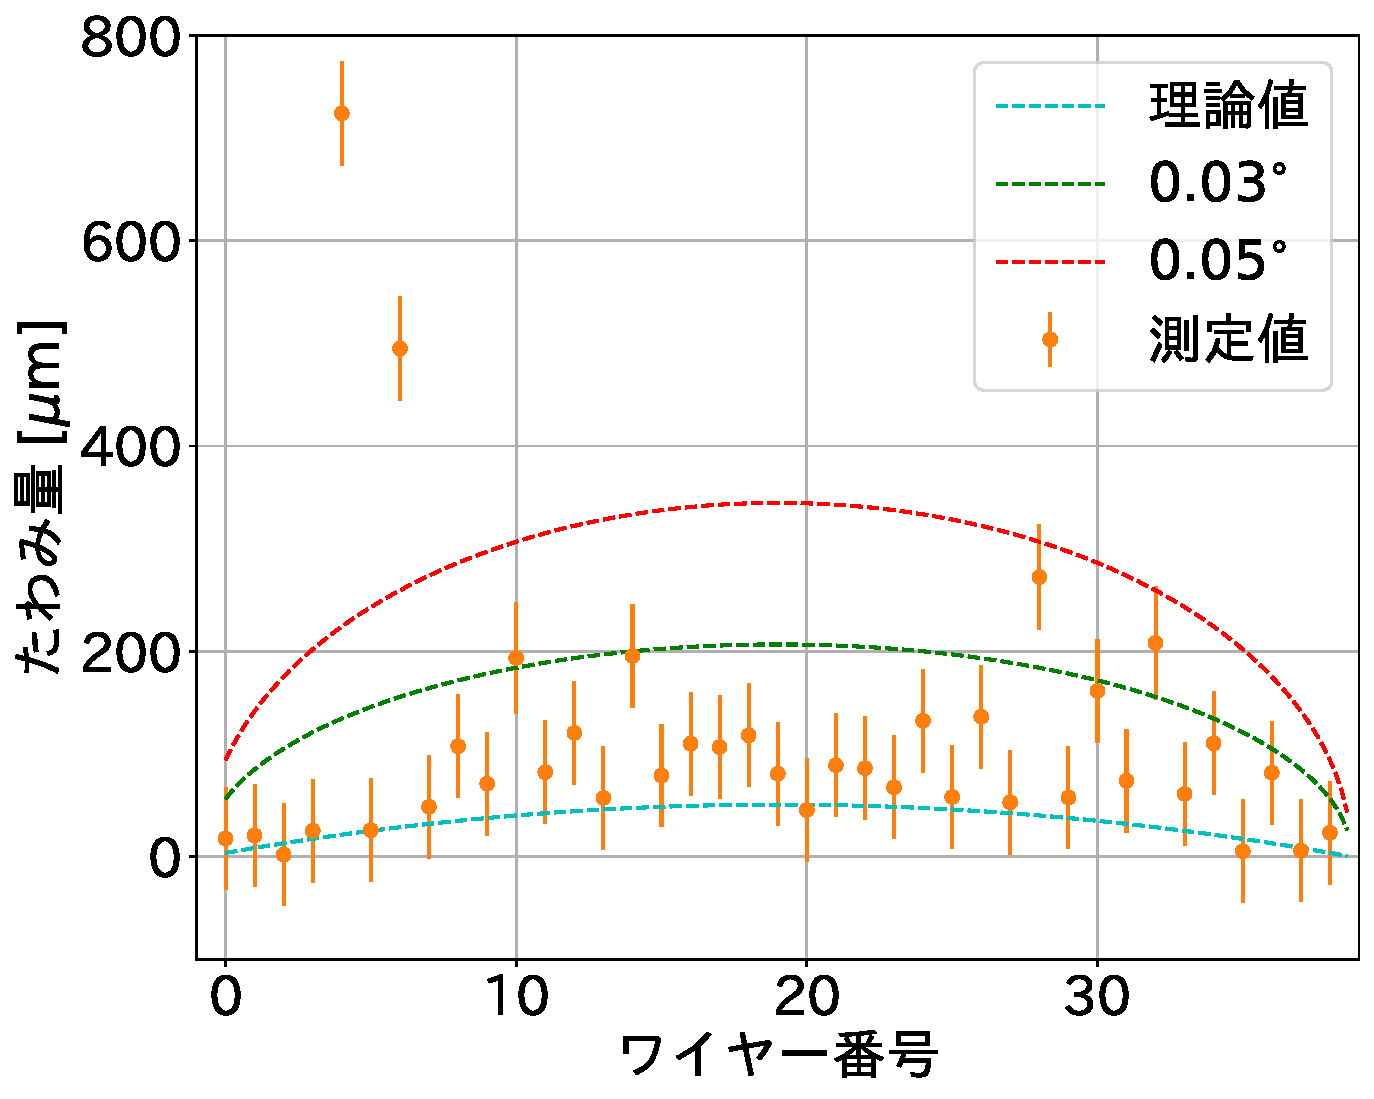
\includegraphics[width=1.0\textwidth]{wiresag_swg/swg_sag_after.pdf}
        \subcaption{}
        \label{fig:wiresag_swg_sag_result_repair}
    \end{minipage}
    \begin{minipage}[b]{0.5\hsize}
        \centering
        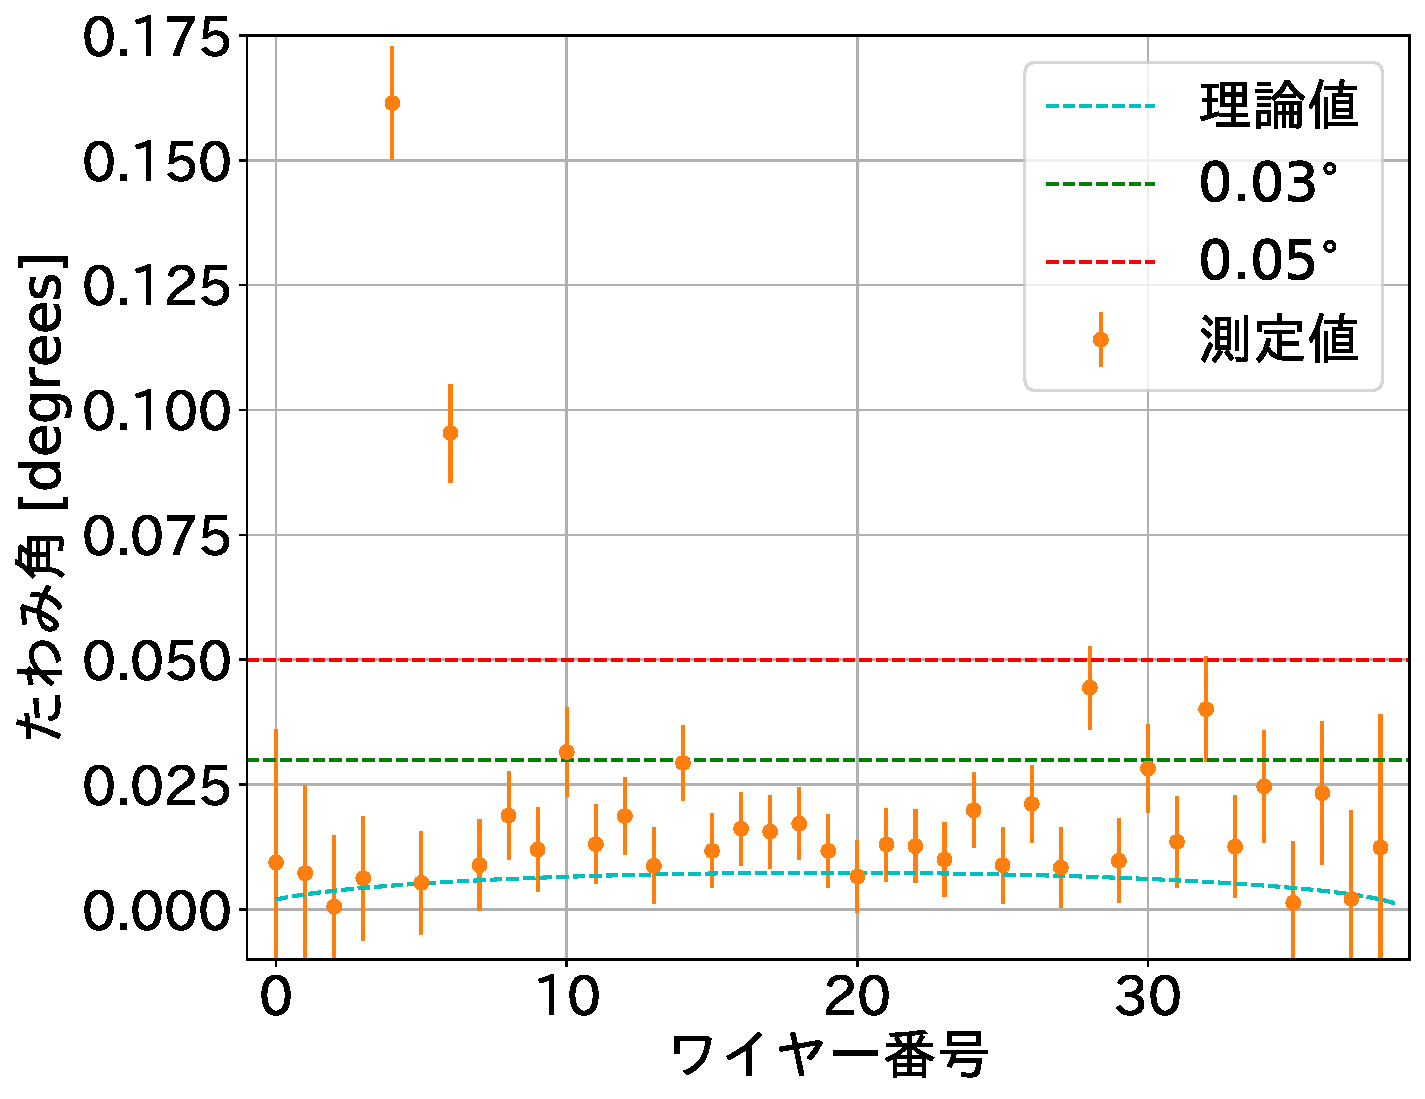
\includegraphics[width=1.0\textwidth]{wiresag_swg/swg_sag_angle_after.pdf}
        \subcaption{}
        \label{fig:wiresag_swg_sag_angle_result_repair}
    \end{minipage}
    \caption{(\subref{fig:wiresag_swg_sag_result_repair}) 修繕後のスパースワイヤーグリッドのたわみ量の評価結果\ 
             (\subref{fig:wiresag_swg_sag_angle_result_repair}) 修繕後のスパースワイヤーグリッドのたわみ角の評価結果}
    \label{fig:wiresag_swg_result_repair}
\end{figure}
\begin{figure}[H]
    \centering
    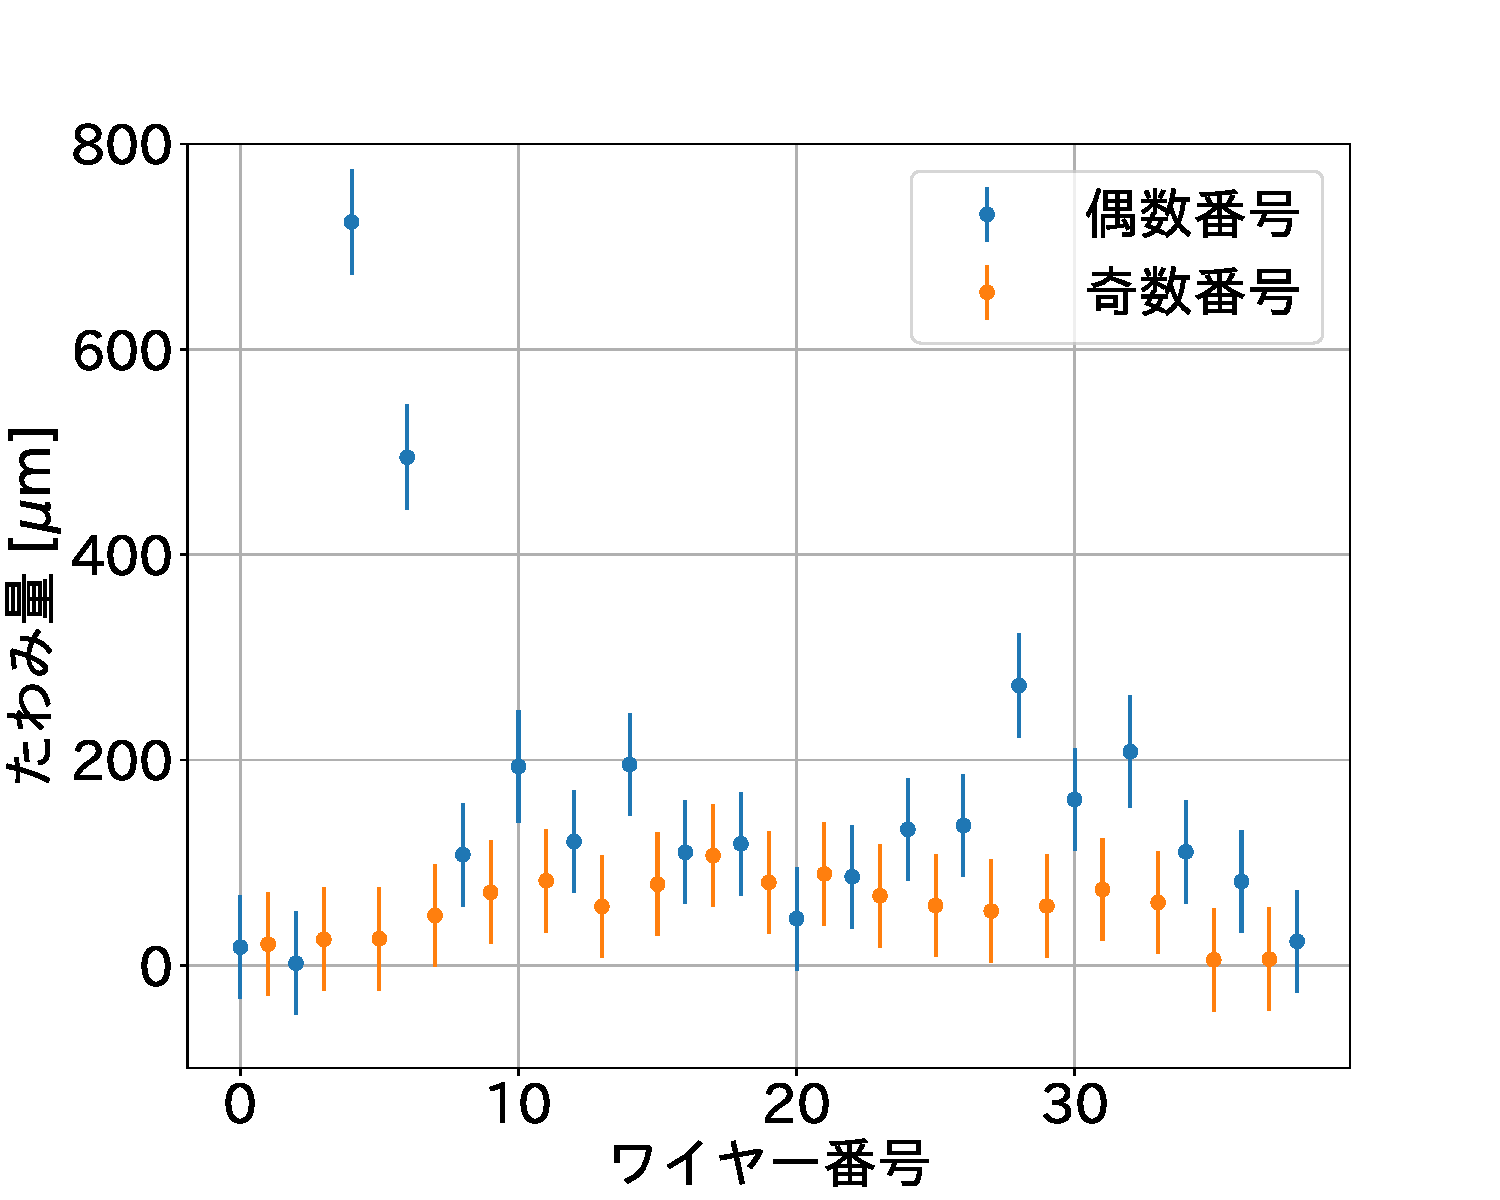
\includegraphics[width=0.8\textwidth]{wiresag_swg/swg_sag_after_even_odd.pdf}
    \caption{修繕後のワイヤー番号の偶奇によるたわみ量の違い}
    \label{fig:wiresag_swg_even_odd_repair}
\end{figure}
\begin{figure}[H]
    \begin{minipage}[b]{0.5\hsize}
        \centering
        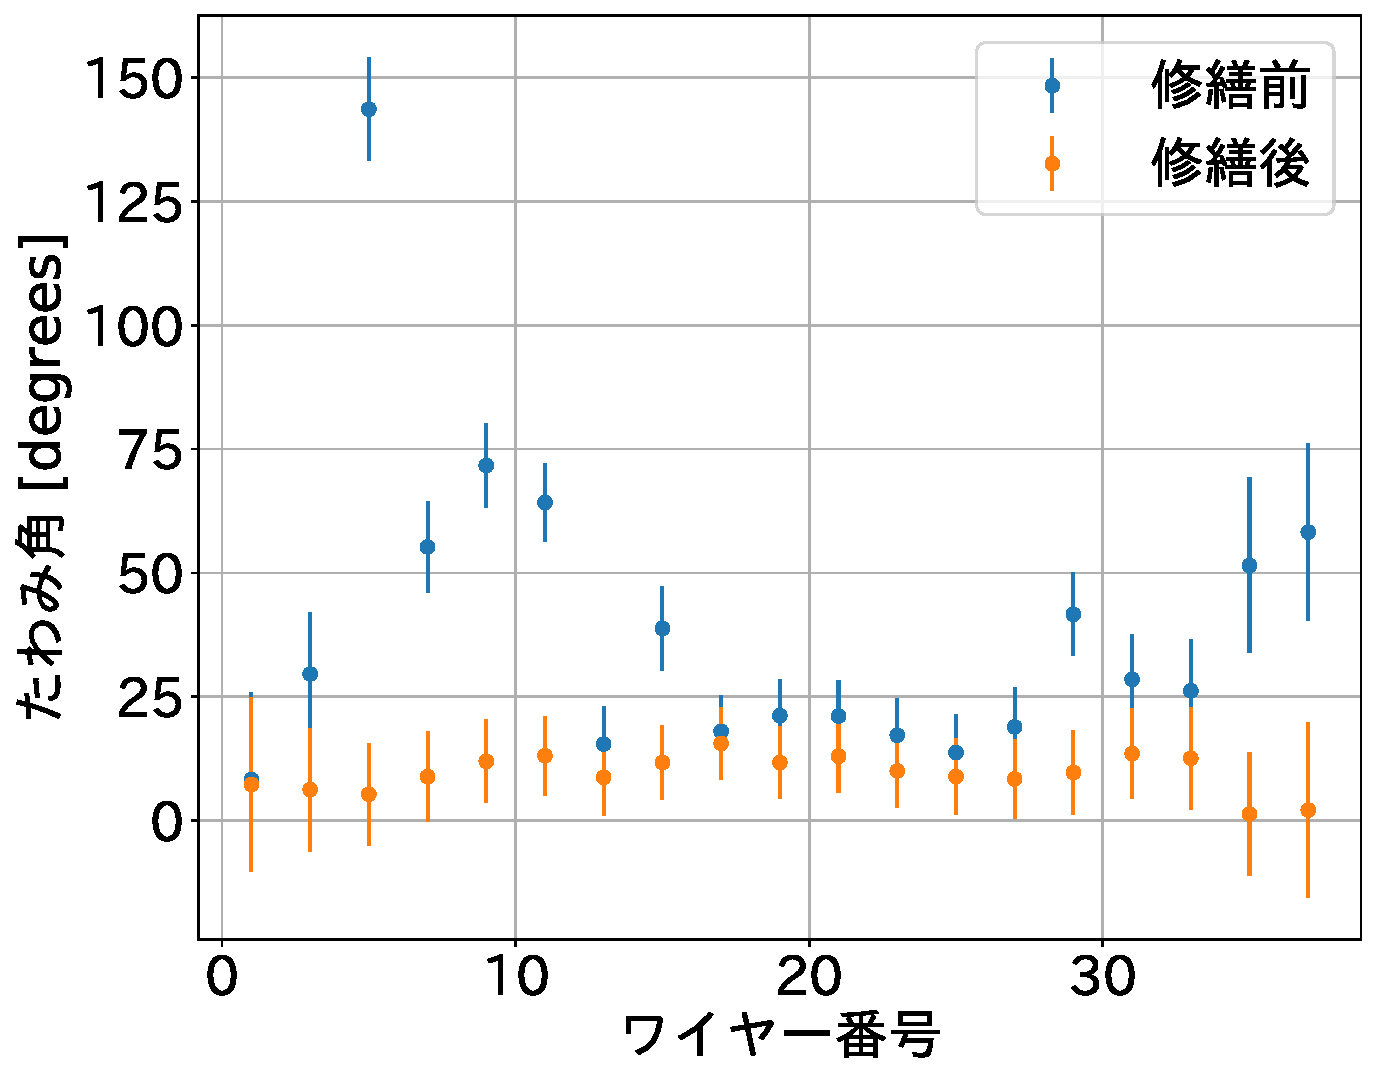
\includegraphics[width=1.0\textwidth]{wiresag_swg/swg_sag_odd_comparison.pdf}
        \subcaption{}
        \label{fig:wiresag_swg_sag_odd_comparison}
    \end{minipage}
    \begin{minipage}[b]{0.5\hsize}
        \centering
        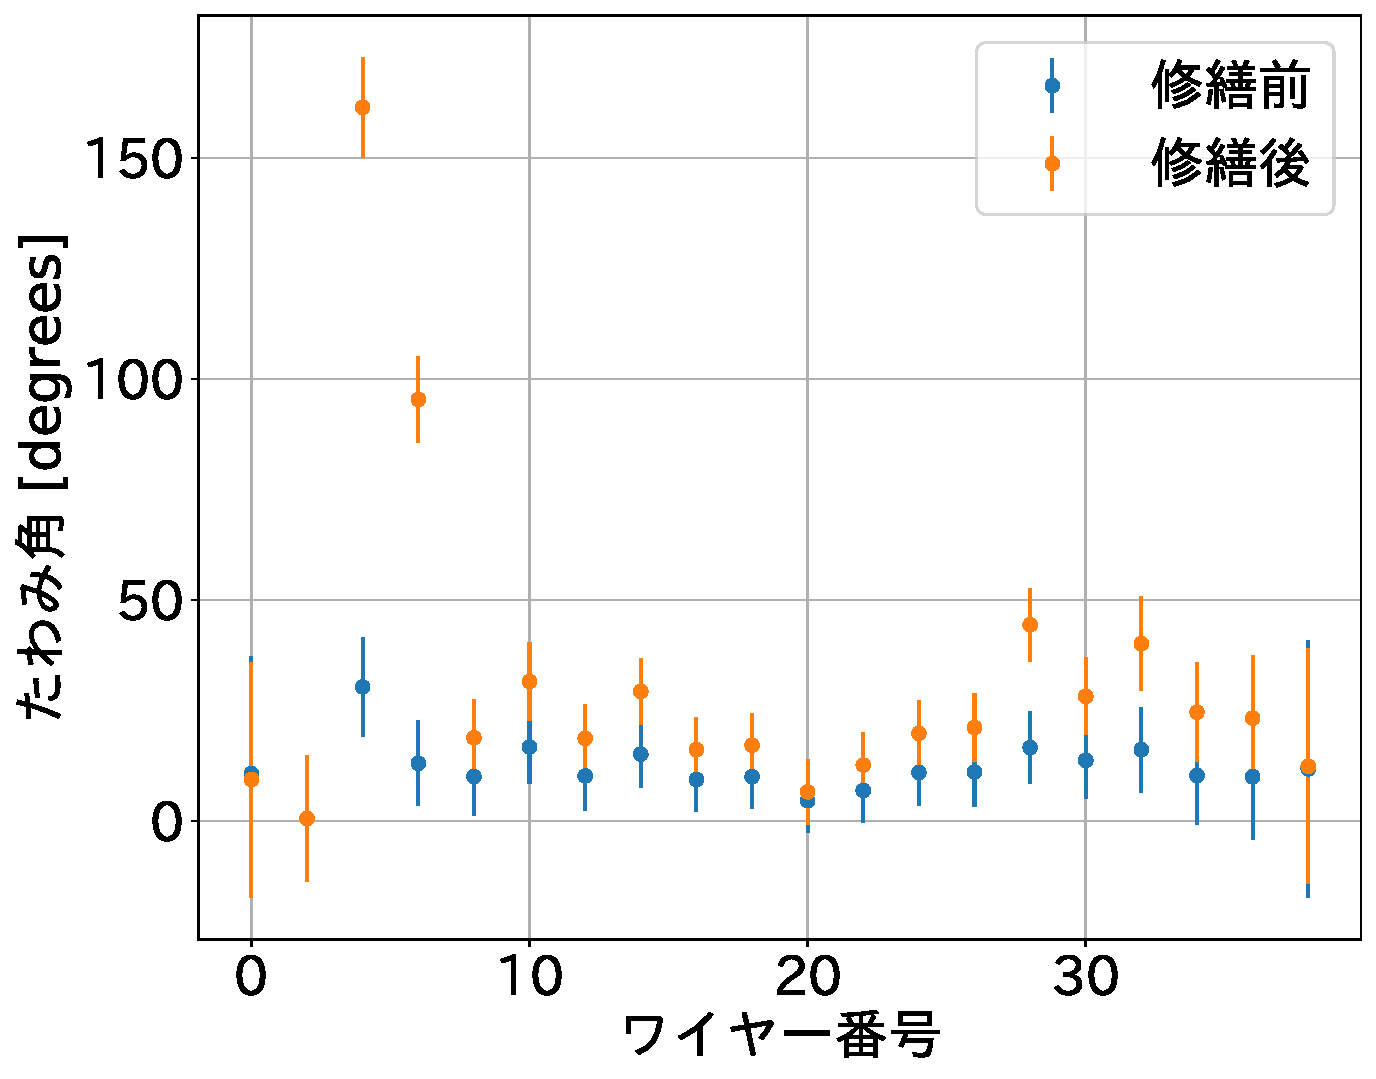
\includegraphics[width=1.0\textwidth]{wiresag_swg/swg_sag_even_comparison.pdf}
        \subcaption{}
        \label{fig:wiresag_swg_sag_even_comparison}
    \end{minipage}
    \caption{(\subref{fig:wiresag_swg_sag_odd_comparison}) 奇数番目のワイヤーのたわみ量の修繕前後での比較\ 
             (\subref{fig:wiresag_swg_sag_even_comparison}) 偶数番目のワイヤーのたわみ量の修繕前後での比較}
    \label{fig:wiresag_swg_even_odd_repair_comparison}
\end{figure}

\section{まとめ}
本章では、開発したワイヤーのたわみ量の自動評価装置を用いて、望遠鏡の偏光角較正に使用されるスパースワイヤーグリッドのたわみ量を評価した。
最初に評価されたワイヤーのたわみ角は$0.036\tcdegree$であったが、評価されたたわみ量が大きいワイヤーを張り直すことでそのたわみ角は$0.03\tcdegree$に改善された。
この評価値は先行研究にて与えられる$<0.05\tcdegree$よりも小さく、本装置を用いて
ワイヤーのたわみ量を改善することでたわみ角を$0.03\tcdegree$程度に抑えることができることが示された。
また、スパースワイヤーグリッドのワイヤーを偶数番目、奇数番目の2回に分けて張ることにより、
先に張られたワイヤーがたわんでしまう可能性があることがわかった。
この原因としては、ワイヤーがスパースワイヤーグリッドのリング部分を歪めている可能性が考えられる。

今後の展望として、たわみ量をさらに抑えるためにはスパースワイヤーグリッドのワイヤーを張る工程を改善することが重要である。
まずはワイヤーをすべて同時に張ることで、ワイヤーのたわみ量を均一に抑えることができるか調べる必要がある。
これによりワイヤーがスパースワイヤーグリッドのリングを歪めているかどうかを検証できる。
また、張力によりワイヤーがスパースワイヤーグリッドのリングを歪めているのであれば、リングの構造を歪みに対して強力なものに変更するか、
ワイヤーにかける張力を弱めることでさらなるたわみ量の改善が見込まれる。

\end{document}